% Source: 2006 Fujian science candidate PDF, source ID
% src-ab0f2729ee4a24495e653b44c14438b4130f8b38b11362bf84251f3595a09d27,
% SHA-256 50d17546b94af82fb2cee653942752914cd387fe72792d74ffa5f75e7a301d83,
% page 1, printed page 288, Q18. Schematic positions only; lengths and angles are not encoded.
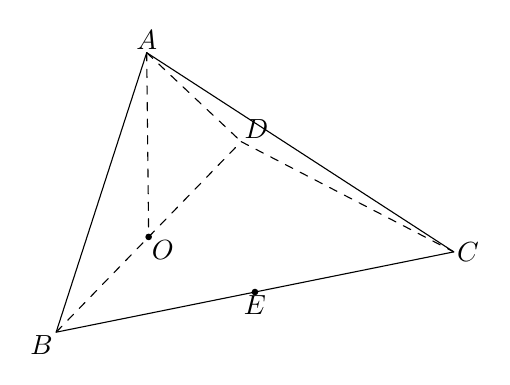
\begin{tikzpicture}[line cap=round,line join=round]
  \coordinate (A) at (1.15,3.55);
  \coordinate (B) at (0,0);
  \coordinate (C) at (5.05,1.02);
  \coordinate (D) at (2.35,2.42);
  \coordinate (O) at (1.175,1.21); % midpoint of BD
  \coordinate (E) at (2.525,0.51); % midpoint of BC

  % Visible and hidden edges of the tetrahedron.
  \draw (A)--(B)--(C)--cycle;
  \draw[dashed] (A)--(D);
  \draw[dashed] (B)--(D);
  \draw[dashed] (D)--(C);
  \draw[dashed] (A)--(O);

  \fill (O) circle (1.2pt);
  \fill (E) circle (1.2pt);
  \node[above,inner sep=1pt]       at (A) {$A$};
  \node[below left,inner sep=1pt]  at (B) {$B$};
  \node[right,inner sep=1pt]       at (C) {$C$};
  \node[above right,inner sep=1pt] at (D) {$D$};
  \node[below right,inner sep=1pt] at (O) {$O$};
  \node[below,inner sep=1pt]       at (E) {$E$};
\end{tikzpicture}
